\documentclass{beamer}

\usepackage{amsmath, amssymb}
\usepackage{graphicx}
\usepackage{url}
\usepackage{xspace}
\usepackage{pifont}
\usepackage{minted}
\usepackage{verbatim}
\usepackage{wasysym}
\usepackage{apacite}

\usetheme{AnnArbor}
\usefonttheme[onlymath]{serif}

\title[Intro DNNs]{\textbf{Practical Deep Neural Networks} \\
\textbf{\normalsize GPU computing perspective}\\
\normalsize Introduction}
\author{Yuhuang Hu \and Chu Kiong Loo}
\institute[UM]{Advanced Robotic Lab\\
Department of Artificial Intelligence\\
Faculty of Computer Science \& IT\\
University of Malaya}

\date{}

\begin{document}

\frame{\titlepage}

\begin{frame}
    \frametitle{Outline}
    \tableofcontents
\end{frame}

\section{Introduction}

\begin{frame}
  \frametitle{Objectives}

  \begin{itemize}
    \item[\ding{226}] Light introduction of numerical computation.
    \item[\ding{226}] Fundamentals of Machine Learning.
    \item[\ding{226}] Support Vector Machine, Softmax Regression.
    \item[\ding{226}] Feed-forward Neural Network.
    \item[\ding{226}] Convolutional Networks.
    \item[\ding{226}] Recurrent Neural Networks.
  \end{itemize} 
\end{frame}

\begin{frame}
  \frametitle{Prerequisites}
    
  \begin{itemize}
  \item[$\star$] Basic training in Calculus 
  \item[$\star$] Basic training in Linear Algebra
    \begin{itemize}
    \item Matrix operations
    \item Matrix properties: transform, rank, norm, determinant, etc
    \item Eigendecomposition, Singular Value Decomposition.
    \end{itemize}
  \item[$\star$] Basic programming skills
    \begin{itemize}
    \item If-else conditioning
    \item Loops
    \item Function, class, library
    \item Source code control: Git (optional)
    \end{itemize}
  \end{itemize}
\end{frame}

\begin{frame}
  \frametitle{References}

  \begin{itemize}
    \item[\ding{169}] Deep Learning: An MIT Press book in preparation

      {\small \emph{Main reference in this workshop, still in development, awesome structure, awesome contents.}}

    \item[\ding{169}] Machine Learning: A probabilistic perspective

      {\small \emph{One of the best Machine Learning books on the market.}}
    \item[\ding{169}] CS231n Convolutional Neural Networks for Visual Recognition Notes

      {\small \emph{Nice structured, well written, loads of pictures.}}

    \item[\ding{169}] CS229 Machine Learning Course Materials

      {\small \emph{For basic knowledge, well written, easy-to-read.}}
  \end{itemize}
\end{frame}

\begin{frame}
    \frametitle{Software and Tools}
    
    \begin{itemize}
        \item[$\star$] Ubuntu 14.04
        \item[$\star$] CUDA Toolkit 7
        \item[$\star$] Python 2.7.9 (Why not 3.*?)
        \item[$\star$] Theano
        \item[$\star$] numpy, scipy, etc
        \item[$\star$] Eclipse+PyDev
    \end{itemize}
\end{frame}

\begin{frame}
  \frametitle{Reading List}

  A reading list is prepared for this workshop, all reading materials can be found at:

  \url{http://rt.dgyblog.com/ref/ref-learning-deep-learning.html}\vspace{1cm}

  \centering\emph{The list keeps expanding!!}
\end{frame}

\section{Machine Learning Prequel}

\subsection{Linear Algebra}

\begin{frame}
    \frametitle{Scalar, Vector, Matrix and Tensor}
\end{frame}

\begin{frame}
    \frametitle{Matrix Operations}
\end{frame}

\begin{frame}
    \frametitle{Matrix Properties}
\end{frame}

\begin{frame}
    \frametitle{Singular Value Decomposition (SVD)}
\end{frame}

\subsection{Basic concepts}

\begin{frame}
    \frametitle{Optimization Problem: Hypothesis}
\end{frame}

\begin{frame}
    \frametitle{Optimization Problem: Cost function}
\end{frame}

\begin{frame}
    \frametitle{Dataset: How to split the data?}
\end{frame}

\begin{frame}
    \frametitle{Dataset: Cross validation}
\end{frame}

\section{Dataset Preparation}

\begin{frame}
    \frametitle{MNIST}
\end{frame}

\begin{frame}
    \frametitle{CIFAR-10}
\end{frame}

\section{Preprocessing}

\subsection{Data Standardization}

\begin{frame}
    \frametitle{Mean subtraction}
\end{frame}

\begin{frame}
    \frametitle{Unit variance}
\end{frame}

\subsection{Principle Components Analysis}

\begin{frame}
    \frametitle{PCA}
\end{frame}

\subsection{ZCA Whitening}

\begin{frame}
    \frametitle{ZCA Whitening}
\end{frame}

\section{Gradient-based Optimization}

\begin{frame}
    \frametitle{SGD}
\end{frame}

\begin{frame}
    \frametitle{Jacobian}
\end{frame}

\begin{frame}
    \frametitle{Hessian}
\end{frame}

\section{Q\&A}

\begin{frame}
  \frametitle{Q\%A}
  
  \begin{figure}
    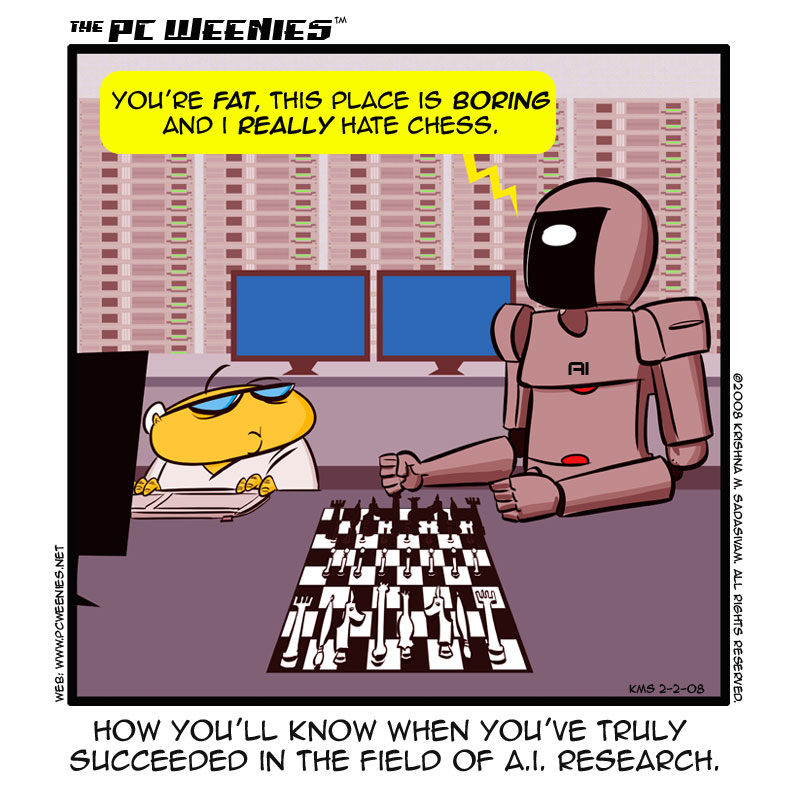
\includegraphics[width=0.6\textwidth]{ai_jokes.jpg}
  \end{figure}
\end{frame}

\end{document}
%%% Local Variables:
%%% mode: latex
%%% TeX-master: t
%%% End:
